%% Springer Nature LaTeX template v3.1 (December 2024), sn-jnl class.
%% Build:  cd paper/springer && pdflatex main && bibtex main && pdflatex main && pdflatex main
%% Body sections are generated from the paper kit (paper/*.md) by convert.py; edit the markdown and re-run it.
%% IJCV instructions: Springer Nature template with the [iicol] option; name-year citations (sn-basic, Springer's
%% author-year style; the APA option needs apacite, which this TeX installation lacks); abstract 150-250 words;
%% 4-6 keywords; 'Statements and Declarations' section; no subfolders in the uploaded source (see make_submission.py).

\documentclass[pdflatex,sn-basic,iicol]{sn-jnl}

\usepackage{graphicx}
\usepackage{multirow}
\usepackage{amsmath,amssymb,amsfonts}
\usepackage{amsthm}
\usepackage{mathrsfs}
\usepackage[title]{appendix}
\usepackage{xcolor}
\usepackage{textcomp}
\usepackage{manyfoot}
\usepackage{booktabs}
\usepackage{longtable}
\usepackage{array}
\usepackage{calc}
\usepackage[T1]{fontenc}
\usepackage{newunicodechar}

%% pandoc helpers used by the generated sections
\providecommand{\tightlist}{\setlength{\itemsep}{0pt}\setlength{\parskip}{0pt}}
\providecommand{\pandocbounded}[1]{#1}
\makeatletter
\def\maxwidth{\ifdim\Gin@nat@width>\linewidth\linewidth\else\Gin@nat@width\fi}
\def\maxheight{\ifdim\Gin@nat@height>\textheight\textheight\else\Gin@nat@height\fi}
\makeatother
\setkeys{Gin}{width=\maxwidth,height=\maxheight,keepaspectratio}
\newcommand{\real}[1]{#1}

%% characters used in the markdown that pdflatex cannot set directly
\newunicodechar{α}{\ensuremath{\alpha}}
\newunicodechar{ε}{\ensuremath{\varepsilon}}
\newunicodechar{ρ}{\ensuremath{\rho}}
\newunicodechar{Δ}{\ensuremath{\Delta}}
\newunicodechar{±}{\ensuremath{\pm}}
\newunicodechar{×}{\ensuremath{\times}}
\newunicodechar{÷}{\ensuremath{\div}}
\newunicodechar{≈}{\ensuremath{\approx}}
\newunicodechar{≤}{\ensuremath{\leq}}
\newunicodechar{≥}{\ensuremath{\geq}}
\newunicodechar{−}{\ensuremath{-}}
\newunicodechar{→}{\ensuremath{\rightarrow}}
\newunicodechar{←}{\ensuremath{\leftarrow}}
\newunicodechar{↔}{\ensuremath{\leftrightarrow}}
\newunicodechar{‖}{\ensuremath{\Vert}}
\newunicodechar{²}{\ensuremath{^{2}}}
\newunicodechar{⁴}{\ensuremath{^{4}}}
\newunicodechar{⁵}{\ensuremath{^{5}}}
\newunicodechar{⁶}{\ensuremath{^{6}}}
\newunicodechar{⁻}{\ensuremath{^{-}}}
\newunicodechar{₀}{\ensuremath{_{0}}}
\newunicodechar{·}{\ensuremath{\cdot}}
\newunicodechar{§}{\S}
\newunicodechar{¶}{\P}

\theoremstyle{thmstyleone}
\newtheorem{theorem}{Theorem}
\newtheorem{proposition}[theorem]{Proposition}
\theoremstyle{thmstyletwo}
\newtheorem{example}{Example}
\newtheorem{remark}{Remark}
\theoremstyle{thmstylethree}
\newtheorem{definition}{Definition}

\raggedbottom

\begin{document}

\title[Zero-initialised connector gates and shortcut learning in VLMs]{A Zero-Initialised Injection Gate Makes Shortcut Learning More Likely in Vision-Language Models}

%% Authors. ORCID iDs are listed in the Declarations (the template's \orcid macro needs an Orcidlogo.eps file
%% that is not in Springer's download); Editorial Manager also collects them at submission.
%% Corresponding-author e-mail: an institutional (sriramachandra.edu.in) address is preferred if available.
\author*[1]{\fnm{Jeyadev} \sur{R}}\email{jeyadev2006@gmail.com}
\author[1]{\fnm{Naveen SomaSekhar Varma} \sur{Vaidani}}

\affil*[1]{\orgdiv{Faculty of Engineering and Technology}, \orgname{Sri Ramachandra Institute of Higher Education and Research}, \orgaddress{\street{No. 1 Ramachandra Nagar, Porur}, \city{Chennai}, \postcode{600116}, \state{Tamil Nadu}, \country{India}}}

\abstract{\textbf{Purpose.} Vision-language models that connect a vision encoder to a language model can rely on
spurious cues such as backgrounds or watermarks. Connectors are compared
on average accuracy alone.
\textbf{Methods.} We hold the language model, frozen vision features, data and training budget fixed and vary only the
connector: a multilayer-perceptron projector, a Q-Former, and gated cross-attention whose tanh injection gate
is learnable from different starts or fixed. We measure worst-group accuracy on three shortcut
tasks with three language models of 3.8B to 9B parameters, on up to fifteen paired seeds.
\textbf{Results.} The zero-initialised gate never opens, although its large gradient changes sign on almost
half the steps, and the model relies on the shortcut while still using the image. Fixing the gate raises
worst-group accuracy by 10.6 and 25.2 points ($d_z$ = 1.10 and 1.34, $p < 0.001$) and removes runs
below 50\%; at 9B the watermark gain doubles to 50.3 points. Gates started open match the fixed gate, smaller starts only partly; a start of 0.01 falls back near zero.
Connector-level reweighting removes the gap on only one task.
With the gate fixed, connector type has no detectable effect, and per-layer gates show no gap. On open-ended question
answering, strong injection harms generation; capping it at the text norm repairs generation but, at 4B, gives back
the watermark robustness gain.
\textbf{Conclusion.} A gate started at or near zero is a controllable architectural cause of shortcut reliance,
injection strength trades robustness against generation quality, and robustness claims need seed-level evaluation.}

\keywords{Shortcut learning, Spurious correlations, Vision-language models, Multimodal large language models, Group robustness, Gated cross-attention}

\maketitle

\section{Introduction}\label{sec:intro}
Vision-language models (VLMs) that connect a pretrained vision encoder to a large language model (LLM) have
become the default way to build general-purpose multimodal systems \cite{yin2024mllmsurvey,zhang2024vlmsurvey,awais2025foundation}. As these systems move into screening, moderation and medical triage, a failure mode
inherited from earlier deep networks becomes critical: \textbf{shortcut learning}, the use of a cue that predicts the
label in training but not in deployment \cite{geirhos2020shortcut}. Shortcuts have already produced high-accuracy
models that read hospital markers instead of lung pathology \cite{degrave2021covid} and watermarks instead of
objects \cite{lapuschkin2019clever}. They fail silently on exactly the under-represented groups where errors are
most costly \cite{brown2023shortcut,ongly2024shortcut}.

A substantial body of work on spurious correlations establishes how to measure and mitigate such failures in
classifiers:
- worst-group accuracy over groups defined by label and spurious attribute \cite{sagawa2020groupdro};
- group-aware or label-free reweighting \cite{liu2021jtt,idrissi2022balancing};
- the finding that features usually retain the core signal, so retraining only the readout recovers most
robustness \cite{izmailov2022feature,kirichenko2023dfr}.

For VLMs, recent studies show that multimodal LLMs inherit spurious cues and fail on minority groups
\cite{hosseini2025spurlens,yang2025spuriverse,zhang2024oodmllm}. They attribute this to the vision encoder
\cite{tong2024eyes}, to data rather than scale \cite{sarridis2026scaling}, or remove it post hoc by unlearning
\cite{sarker2026purge}. In parallel, a separate line of work compares the connectors that map visual features into
the LLM, such as MLP projectors, Q-Formers and gated cross-attention \cite{liu2024llava15,li2023blip2,alayrac2022flamingo}, and ranks them by benchmark accuracy and efficiency \cite{mckinzie2024mm1,cha2024honeybee,karamcheti2024prismatic}.

However, these two lines of work have not met, which leaves three limitations.
1. \textbf{No controlled test of the connector.} Every robustness study of VLMs treats the connector as fixed, and
every connector study measures average accuracy rather than worst-group behaviour. Whether the component
that decides \emph{what visual information reaches the LLM} also decides \emph{whether the model relies on a
shortcut} is untested.
2. \textbf{Conflicting evidence on gated cross-attention.} Zero-initialised, learnable tanh gates are the standard
way to inject a new modality into a pretrained LLM: Flamingo, IDEFICS, LLaMA-Adapter and Llama 3.2 Vision
all use them \cite{alayrac2022flamingo,zhang2024llamaadapter,grattafiori2024llama3}. Cross-attention
injection performs well with frozen backbones \cite{laurencon2024matters}. Yet learnable injection gates can end
up behaviourally closed \cite{farazi2026gate}, and every attention gate in the released Llama 3.2 Vision
checkpoints is below 0.012. The consequence of a near-shut gate for \emph{what the model relies on} has never
been measured. Work on modality imbalance shows that multimodal networks can greedily ignore a modality
\cite{wu2022greedy,huang2022modality}, but not which component of an LLM-based VLM causes it, nor what it does
to spurious-group robustness.
3. \textbf{Results from too few seeds.} Comparisons rest on one or a few training runs, although seed variance
alone can reverse conclusions in deep learning \cite{henderson2018matters,bouthillier2021variance}.

The field therefore cannot say whether a widely used architectural choice silently causes shortcut learning,
or how to avoid it.

To address these limitations, this study tests whether the vision-language connector, and specifically its
injection gate, determines shortcut reliance in LLM-based VLMs.
- \textbf{What is held fixed:} the LLM (Qwen3.5-4B, replicated with Phi-4-mini), frozen SigLIP features, data,
prompts and training budget.
- \textbf{What varies:} only the connector, at four levels: an MLP projector, a Q-Former, and gated
cross-attention with a learnable or a fixed gate. The two gate variants have identical parameters; a third,
learnable gate initialised open separates trainability from initialisation.
- \textbf{Where it is measured:} worst-group accuracy on Waterbirds, a controlled watermark task and CelebA.
- \textbf{How it is tested:} hypotheses formed on a 3-seed pilot and confirmed on up to 12 new paired
seeds (15 in total), with effect sizes,
robust and non-parametric tests, and an equivalence test.
- \textbf{Fixes and rival explanations:} we log the gate during training, read the gates of released IDEFICS
checkpoints, test a connector-only analogue of deep feature reweighting, and probe rival explanations
(token count, encoder scale, frozen LLM, training length).

This paper makes three contributions.
1. \textbf{A transmission mechanism.} We identify the learnable injection gate as a \emph{transmission bottleneck}
between features and readout. Initialised at zero, the gate never opens, and the model then relies on the shortcut; fixing it raises
worst-group accuracy by 10.6 and 25.2 points (d\_z = 1.10 and 1.34). This extends the feature--readout account
of shortcut learning and links gate closure to robustness.
2. \textbf{Variance as an outcome.} The learnable gate turns robustness into a seed lottery, with up to 10 of 15
runs collapsing. Once the gate is fixed, we detect no significant difference between connector types, although equivalence
is not established. Together these establish
that architectural robustness claims require seed-level evaluation.
3. \textbf{A practical fix and its boundary.} Retraining only the connector on a small group-balanced set raises
watermark worst-group accuracy to 89.6\% with near-zero seed variance, but not when the shortcut is entangled
with the object.

Section 2 reviews related work. Section 3 describes the design and statistical protocol. Section 4 reports the
results, Section 5 discusses mechanisms and implications, and Section 6 concludes. Code, per-seed results and
figures are public.


\section{Related work}\label{sec:related}
\subsection{Shortcut learning and group robustness}

Shortcut learning, the reliance on a cue that predicts the label in training but not at deployment, is documented
from medical imaging to watermark detection \cite{geirhos2020shortcut,degrave2021covid,lapuschkin2019clever}. Its
standard measure is worst-group accuracy over groups defined by label and spurious attribute, with Waterbirds and
CelebA as benchmarks \cite{sagawa2020groupdro,liu2015celeba}. Mitigations act on data or training: group-robust
optimisation and balanced sampling \cite{sagawa2020groupdro,idrissi2022balancing}, label-free reweighting
\cite{nam2020lff,liu2021jtt,qiu2023afr}, invariance-seeking objectives \cite{huang2024losingtickets,mitchell2026wule}, and
embedding regularisers that reach high worst-group accuracy with attribute labels \cite{park2026scer}. A key finding is
that features usually retain the core signal, so retraining only the readout recovers most robustness
\cite{izmailov2022feature,kirichenko2023dfr}. This literature studies classifiers: the architecture between features and
readout is not a variable. Our study makes that architecture the variable, and tests a readout-style fix at the
connector.

\subsection{Shortcuts and language priors in vision-language models}

Before LLM-based models, VQA systems answered from question priors, which VQA-CP was built to expose
\cite{agrawal2018vqacp,goyal2019vqav2}. Contrastive models such as CLIP carry spurious correlations and read rendered
text \cite{radford2021clip,materzynska2022disentangling}, and fixes act on adapters, prompts or calibration
\cite{zhang2022adapters,chuang2023biasedprompts,you2024calibrating}. For MLLMs, benchmarks show reliance on spurious cues
and poor generalisation beyond them \cite{hosseini2025spurlens,yang2025spuriverse,ye2026mmspubench,zhang2024oodmllm},
and robustness under shift remains open for vision-language alignment \cite{zhu2024vlalignood}. The proposed causes are the
vision encoder \cite{tong2024eyes}, data rather than scale \cite{sarridis2026scaling}, or are removed after training
\cite{sarker2026purge}. A gating unit that keeps language from fusing directly into visual features reduces language
shortcuts in a CLIP-based video QA model \cite{zou2024videodistill}, and an entity-grounded gate improves cross-domain
robustness of an MLLM adapter \cite{ahn2026evident}. None of these varies the connector of an LLM-based VLM as a
controlled factor.

\subsection{Connector design}

Three connector families dominate \cite{yin2024mllmsurvey,huang2025vitsurvey}: projection (MLP projectors
\cite{liu2024llava15}), query-based (the Q-Former \cite{li2023blip2}) and gated cross-attention (Flamingo, IDEFICS and the
Llama 3.2 vision adapters \cite{alayrac2022flamingo,laurencon2023obelics,grattafiori2024llama3}). Design studies rank
connectors by benchmark accuracy and efficiency \cite{mckinzie2024mm1,cha2024honeybee,karamcheti2024prismatic,tong2024cambrian} and find that connector type matters less than token count and resolution \cite{mckinzie2024mm1}. The only
three-way comparison we found on another outcome, cross-modal unlearning, compares released models that also differ
in encoder, LLM and size \cite{balaji2026forget}. Surveys list robustness and bias as open challenges for MLLMs
\cite{awais2025foundation,zhang2024vlmsurvey}, but no design study measures them.

\subsection{Gated injection and initialisation}

Zero-initialised learnable scales let a new branch start as the identity: ReZero and SkipInit for residual blocks
\cite{bachlechner2021rezero,de2020skipinit}, LayerScale with a small non-zero start that trains better than zero
\cite{touvron2021cait}, and LLaMA-Adapter and Flamingo for adding a modality to a frozen LLM \cite{zhang2024llamaadapter,alayrac2022flamingo}. Farazi et al.~show that learnable gates on image-derived pathways in frozen VLMs settle near
zero and become behaviourally closed; they explain this by a vanishing first-order gradient when the injected signal
does not depend on the caption, recommend injecting at matched norm without a gate, and leave text-coupled injection
and gate initialisation untested \cite{farazi2026gate}. Li et al.~show that visual tokens with much larger norms than
text tokens lose information in pre-norm MLLMs \cite{li2025unseen}. Modality-imbalance work finds that multimodal
networks greedily under-use one modality, with the winner depending on initialisation, and corrects it by gradient
modulation \cite{wu2022greedy,huang2022modality,peng2022balanced}. We bring these lines together: we vary the gate's
start value in a text-coupled connector and measure the consequence for shortcut reliance.

\subsection{Evaluation practice}

Seed variance alone can reverse deep-learning conclusions \cite{henderson2018matters,bouthillier2021variance,picard2021seed}, and model selection changes robustness results \cite{gulrajani2021domainbed}. We therefore state
hypotheses on a pilot, confirm them on new paired seeds, correct for multiple tests \cite{holm1979simple}, report effect
sizes and equivalence tests \cite{schuirmann1987tost}, and treat seed-level collapse as an outcome.


\section{Methods}\label{sec:methods}
\subsection{Research design and paradigm}

\textbf{Design.}
- The study is a \textbf{controlled, between-architecture experiment with repeated randomised runs}: a full
factorial over connector × task with seeds as replicates, plus targeted follow-ups.
- Only one factor varies at a time: the vision-language connector, or one specified follow-up factor.
- Everything else is held fixed: the LLM, the frozen vision features, the data, the prompt, the optimiser and
the training budget.

\textbf{Why this design.}
- The research question is causal: \emph{does the connector change shortcut reliance?}
- Observational comparisons of released VLMs cannot answer it, because released models differ in data, scale,
encoder and training recipe at the same time.
- Design studies of VLMs \cite{mckinzie2024mm1,karamcheti2024prismatic} show that only controlled ablations can
attribute effects to one component.
- Seed-level replication is required because a single seed can reverse conclusions in deep learning
\cite{henderson2018matters,picard2021seed,bouthillier2021variance}.

\textbf{Paradigm.}
- The study is positivist and hypothesis-testing.
- The primary hypotheses (H1, H2), their tests, the significance level (one-sided α = 0.025) and the
equivalence margin (±3 WGA points) were written down before the seed-extension runs (see
\href{OUTLINE.md}{\texttt{OUTLINE.md}} and \href{../study/hypotheses.py}{\texttt{study/hypotheses.py}}).
- Analyses beyond these are labelled exploratory.

\subsection{Data sources, sampling and inclusion criteria}

{\def\LTcaptype{none} % do not increment counter
\begin{longtable}[]{@{}
  >{\raggedright\arraybackslash}p{(\linewidth - 12\tabcolsep) * \real{0.1290}}
  >{\raggedright\arraybackslash}p{(\linewidth - 12\tabcolsep) * \real{0.1290}}
  >{\raggedright\arraybackslash}p{(\linewidth - 12\tabcolsep) * \real{0.1290}}
  >{\raggedright\arraybackslash}p{(\linewidth - 12\tabcolsep) * \real{0.1290}}
  >{\centering\arraybackslash}p{(\linewidth - 12\tabcolsep) * \real{0.1613}}
  >{\centering\arraybackslash}p{(\linewidth - 12\tabcolsep) * \real{0.1613}}
  >{\centering\arraybackslash}p{(\linewidth - 12\tabcolsep) * \real{0.1613}}@{}}
\toprule\noalign{}
\begin{minipage}[b]{\linewidth}\raggedright
Task
\end{minipage} & \begin{minipage}[b]{\linewidth}\raggedright
Source
\end{minipage} & \begin{minipage}[b]{\linewidth}\raggedright
Shortcut (spurious attribute \emph{a})
\end{minipage} & \begin{minipage}[b]{\linewidth}\raggedright
Label \emph{y}
\end{minipage} & \begin{minipage}[b]{\linewidth}\centering
Train
\end{minipage} & \begin{minipage}[b]{\linewidth}\centering
Val
\end{minipage} & \begin{minipage}[b]{\linewidth}\centering
Test
\end{minipage} \\
\midrule\noalign{}
\endhead
\bottomrule\noalign{}
\endlastfoot
Waterbirds & CUB-200 birds on Places backgrounds \cite{wah2011cub,zhou2018places}, official splits \cite{sagawa2020groupdro} & background (land / water) & landbird / waterbird & 4,795 & 1,199 & 5,794 \\
Watermark (ours) & MS-COCO images \cite{lin2014coco} & stock-photo text watermark in the corner & dog present & 4,800 (95\% shortcut-aligned) & 1,200 (group-balanced) & 2,400 (group-balanced) \\
CelebA & CelebA, official partitions \cite{liu2015celeba} & gender (Male) & Blond\_Hair & 8,000 (stratified subsample) & 5,000 (≥ 100 per group) & full official test \\
VQA-CP v2 (open-ended) & VQA-CP v2 \cite{agrawal2018vqacp} on COCO images & question-type answer prior (text side) & free-form answer & 8,000 questions from the VQA-CP train split & 1,000 (same split, in-distribution) & 2,000 in-distribution + 3,000 from the VQA-CP test split (shifted priors); image-disjoint \\
Alignment captions & MS-COCO captions & -- & -- & 10,000 pairs & -- & -- \\
\end{longtable}
}

\textbf{Sampling.}
- \emph{Waterbirds:} official splits, kept unchanged for comparability with the group-robustness literature
\cite{sagawa2020groupdro,kirichenko2023dfr}.
- \emph{Watermark:}
- Training uses stratified sampling with 95\% of examples shortcut-aligned (watermark ↔ dog), the same
strength as Waterbirds.
- Validation and test are \textbf{group-balanced}, so every group is measured with equal precision.
- All splits are deterministic (\texttt{study/build\_tasks.py}, seed 0).
- \emph{CelebA:} train and validation are stratified subsamples that preserve group proportions, to fit the
compute budget; the official test set is used in full.

\textbf{Inclusion and exclusion.}
- Alignment captions exclude every image in any task's validation or test split, to prevent leakage.
- The Watermark label comes from the COCO object annotations: an image is positive if any annotation is
``dog''.
- No run was excluded after the fact. Runs that crashed (out-of-memory, session limits) were re-run with the
same seed, and every finished run is reported (\texttt{results\_study/*/all\_runs.csv}).

\textbf{Power analysis (sample size = seeds).}
- The unit of replication is the training seed. Each seed varies data order, LoRA initialisation and
stage-2 sampling \cite{bouthillier2021variance}.
- Power for the one-sided paired t-test at α = 0.025 was computed from the non-central t distribution
\cite{cohen1988power}.

{\def\LTcaptype{none} % do not increment counter
\begin{longtable}[]{@{}
  >{\centering\arraybackslash}p{(\linewidth - 10\tabcolsep) * \real{0.1667}}
  >{\centering\arraybackslash}p{(\linewidth - 10\tabcolsep) * \real{0.1667}}
  >{\centering\arraybackslash}p{(\linewidth - 10\tabcolsep) * \real{0.1667}}
  >{\centering\arraybackslash}p{(\linewidth - 10\tabcolsep) * \real{0.1667}}
  >{\centering\arraybackslash}p{(\linewidth - 10\tabcolsep) * \real{0.1667}}
  >{\centering\arraybackslash}p{(\linewidth - 10\tabcolsep) * \real{0.1667}}@{}}
\toprule\noalign{}
\begin{minipage}[b]{\linewidth}\centering
Paired effect size d\_z
\end{minipage} & \begin{minipage}[b]{\linewidth}\centering
Power with 3 seeds
\end{minipage} & \begin{minipage}[b]{\linewidth}\centering
5 seeds
\end{minipage} & \begin{minipage}[b]{\linewidth}\centering
10 seeds
\end{minipage} & \begin{minipage}[b]{\linewidth}\centering
15 seeds
\end{minipage} & \begin{minipage}[b]{\linewidth}\centering
Seeds for 80\% power
\end{minipage} \\
\midrule\noalign{}
\endhead
\bottomrule\noalign{}
\endlastfoot
0.8 (large) & 0.13 & 0.28 & 0.62 & 0.82 & 15 \\
1.0 & 0.18 & 0.40 & 0.80 & 0.95 & 10 \\
1.5 & 0.32 & 0.71 & 0.99 & 1.00 & 6 \\
2.0 & 0.47 & 0.91 & 1.00 & 1.00 & 5 \\
\end{longtable}
}

The initial 3-seed design had power below 0.5 even for large effects. The gate comparison was therefore
extended to \textbf{15 seeds per arm on both tasks}, enough for 80\% power at d\_z ≥ 0.8. Observed effects
(Section 4 of the results) are d\_z = 1.10 and 1.34, giving achieved power of 0.98 and \textgreater{} 0.99. Phi-4-mini
Watermark (d\_z ≈ 1.0, power 0.40 at 5 seeds) was extended to 10 seeds \emph{after} its 5-seed test missed
α = 0.025 (p = 0.044). This data-dependent extension is disclosed, and the new seeds 5--9 are also tested on
their own as fresh data (p = 0.023).

\subsection{Variables and instrumentation}

\textbf{Independent variable: connector}, four levels:

{\def\LTcaptype{none} % do not increment counter
\begin{longtable}[]{@{}
  >{\raggedright\arraybackslash}p{(\linewidth - 6\tabcolsep) * \real{0.2222}}
  >{\raggedright\arraybackslash}p{(\linewidth - 6\tabcolsep) * \real{0.2222}}
  >{\centering\arraybackslash}p{(\linewidth - 6\tabcolsep) * \real{0.2778}}
  >{\centering\arraybackslash}p{(\linewidth - 6\tabcolsep) * \real{0.2778}}@{}}
\toprule\noalign{}
\begin{minipage}[b]{\linewidth}\raggedright
Level
\end{minipage} & \begin{minipage}[b]{\linewidth}\raggedright
Design
\end{minipage} & \begin{minipage}[b]{\linewidth}\centering
Image tokens
\end{minipage} & \begin{minipage}[b]{\linewidth}\centering
Trainable params
\end{minipage} \\
\midrule\noalign{}
\endhead
\bottomrule\noalign{}
\endlastfoot
MLP projector \cite{liu2024llava15} & LayerNorm--Linear--GELU--Linear over 2×2-pooled patches & 49 & 8.5M \\
Q-Former \cite{li2023blip2} & 32 learned queries, 8 heads, 1 block & 32 & 11.4M \\
Cross-attention, learned gate \cite{alayrac2022flamingo} & prompt tokens attend to patches; \texttt{e\ ←\ e\ +\ tanh(α)·attn}, α₀ = 0 & 0 & 8.9M \\
Cross-attention, fixed gate & identical block; gate fixed open, output layer zero-initialised & 0 & 8.9M \\
\end{longtable}
}

The two cross-attention levels have the \textbf{same parameters and FLOPs}; only whether \texttt{α} is trainable
differs. Both start as the identity map. This isolates the gate as the manipulated mechanism and removes
capacity as a rival explanation.

\textbf{Dependent variables.}
- \textbf{Primary: test worst-group accuracy (WGA)} \cite{sagawa2020groupdro}.
- Mean over three question phrasings, one of them never seen in training.
- Checkpoint chosen by validation WGA.
- \textbf{Secondary:}
- average accuracy: the plain mean over test images. It is \emph{not} reweighted to the training-group
frequencies, as some Waterbirds papers do \cite{sagawa2020groupdro}, so it is not directly comparable to their
``average accuracy'';
- ID and OOD accuracy and their gap \cite{koh2021wilds};
- balanced accuracy;
- seed variance of WGA (H2);
- WGA with the label-free checkpoint rule (validation average accuracy).
- \textbf{Mechanism measures:} the learned gate value \texttt{tanh(α)} and its gradient, logged every 10 alignment steps.
Up to round 4 the logged gradient is the value after global-norm clipping at 1 (as in Flamingo); from round 5
the raw pre-clip gradient and the pre-clip global norm are logged as well (\texttt{grad\_raw}, \texttt{grad\_norm\_total}).
- \textbf{Behavioural pathway test:} from round 5, every selected checkpoint is re-tested with the connector's visual
contribution removed (\texttt{ablated\_mean\_over\_templates}). If WGA does not change, the pathway is behaviourally
closed, the criterion of \cite{farazi2026gate}.
Also the share of attention on the watermark corner.

\textbf{Controlled variables, and why each is controlled.}
- \textbf{LLM:} Qwen3.5-4B \cite{qwen2026qwen35}, NF4 4-bit with LoRA r = 16 \cite{dettmers2023qlora,hu2022lora}.
Controlled because LLM capacity and pretraining change shortcut reliance \cite{sagawa2020overparam}. Varied once
(Phi-4-mini \cite{abouelenin2025phi4mini}) to test generality.
- \textbf{Vision features:} frozen SigLIP \cite{zhai2023siglip}, cached once, so every connector receives
bit-identical inputs. Encoder choice strongly affects MLLMs \cite{tong2024cambrian,tong2024eyes}. Varied once
(SigLIP-large).
- \textbf{Data, prompts and answer read-out:}
- The same splits, the same chat template and the same 2 training phrasings for every connector.
- The prediction is the more likely of the two answer tokens, which removes free-text parsing as a
confounder.
- \textbf{Optimisation and budget:}
- \emph{Stage 1:} 300 alignment steps on 10k COCO captions with the LLM frozen.
- \emph{Stage 2:} 4 epochs, batch 16, learning rate 2e-4, cosine schedule.
- The same for every connector, with early stopping after 2 epochs without validation-WGA gain.
- The budget is equalised in steps, not wall-clock time, so faster connectors gain no extra training.
- \textbf{Image-token count:} differs by design (49 / 32 / 0). It is checked with a 36-token MLP ablation,
because token count is a known design factor \cite{cha2024honeybee,mckinzie2024mm1}.

\subsection{Procedure}

\begin{enumerate}
\def\labelenumi{\arabic{enumi}.}
\tightlist
\item
  \textbf{Data preparation} (\texttt{study/build\_tasks.py}, \texttt{study/cache\_features.py}): build splits and cache frozen
  patch features (one Kaggle CPU/GPU session per encoder).
\item
  \textbf{Stage 1, alignment} (\texttt{study/align.py}): train only the connector on COCO captions, with the LLM frozen.
  This follows the two-stage practice of \cite{liu2023llava,liu2024llava15}. 300 steps suffice because alignment
  is coarse and data-efficient \cite{groger2026rethinking}.
\item
  \textbf{Stage 2, task training} (\texttt{study/train\_task.py}): train LoRA and the connector on each task under ERM
  with natural (shortcut-biased) sampling.
\item
  \textbf{Stage 3, optional connector-only fixes:} freeze the LLM and LoRA, then retrain only the connector:

  \begin{itemize}
  \tightlist
  \item
    \textbf{Connector-DFR:} on a group-balanced half of validation, the other half selecting the model
    \cite{kirichenko2023dfr}.
  \item
    \textbf{Connector-JTT:} stage-2 errors upweighted ×20 \cite{liu2021jtt}.
  \end{itemize}
\item
  \textbf{Evaluation:}

  \begin{itemize}
  \tightlist
  \item
    Test metrics for each phrasing.
  \item
    Per-image predictions saved (\texttt{arrays.npz}) for the bootstrap.
  \item
    \texttt{environment.txt} (exact package versions and GPU) written next to every result.
  \end{itemize}
\item
  \textbf{Execution:}

  \begin{itemize}
  \tightlist
  \item
    Runs on Kaggle (2× NVIDIA T4, 16 GB), one job per GPU.
  \item
    Jobs are resumable; results are exported after every run.
  \item
    Seeds were assigned before the runs; no run was selected after seeing its result.
  \end{itemize}
\end{enumerate}

\textbf{Bias-minimisation steps.}
- Identical code paths for all connectors: one \texttt{train\_task.py} with a \texttt{-\/-connector} flag.
- A held-out question phrasing is used to detect prompt over-fitting.
- Two checkpoint-selection rules are reported: one uses group labels, one does not.
- Group-label use is stated for every method.
- The full per-seed results are released.

\subsection{Analysis strategy}

{\def\LTcaptype{none} % do not increment counter
\begin{longtable}[]{@{}
  >{\raggedright\arraybackslash}p{(\linewidth - 4\tabcolsep) * \real{0.3333}}
  >{\raggedright\arraybackslash}p{(\linewidth - 4\tabcolsep) * \real{0.3333}}
  >{\raggedright\arraybackslash}p{(\linewidth - 4\tabcolsep) * \real{0.3333}}@{}}
\toprule\noalign{}
\begin{minipage}[b]{\linewidth}\raggedright
Question
\end{minipage} & \begin{minipage}[b]{\linewidth}\raggedright
Test
\end{minipage} & \begin{minipage}[b]{\linewidth}\raggedright
Why this test
\end{minipage} \\
\midrule\noalign{}
\endhead
\bottomrule\noalign{}
\endlastfoot
H1: fixed \textgreater{} learned gate & One-sided \textbf{paired t-test} over seeds, with a \textbf{Wilcoxon signed-rank} test as the assumption-free check \cite{dror2018hitchhiker}; \textbf{Holm} correction across the four H1 cells (2 LLMs × 2 tasks); unpaired Welch and Mann--Whitney tests as checks & Seeds pair the two arms (same data order and initialisation), removing between-seed variance \\
H2: learned gate more variable & One-sided \textbf{variance-ratio F-test}, with the \textbf{Brown--Forsythe} test as a robust check, and \textbf{Fisher's exact test} on the number of collapsed runs (WGA \textless{} 50) & The F-test is sensitive to non-normality; Brown--Forsythe is not; the collapse count tests the practical claim directly \\
Pairwise connector differences & \textbf{Stratified bootstrap} of test images (2,000 resamples) and a \textbf{hierarchical bootstrap} over seeds and images \cite{efron1993bootstrap}; \textbf{Holm--Bonferroni} correction within each task \cite{holm1979simple} & The hierarchical bootstrap covers training variance, not just test-sample noise \\
``Connector type does not matter'' & \textbf{Two one-sided tests (TOST)}, margin ±3 points \cite{schuirmann1987tost} & A non-significant difference is not evidence of equivalence \\
Effect size & Paired \textbf{Cohen's d\_z} (mean difference / s.d. of differences), plus d\_av for comparison across designs \cite{cohen1988power} & p-values alone do not show practical importance \\
\end{longtable}
}

\textbf{Confirmatory vs exploratory.} Only the four H1 tests (2 LLMs × 2 tasks, Holm-corrected) and H2 on
Qwen3.5-4B are confirmatory. Every control (open and half-open gate, learning rate, alignment length, Group DRO,
injection ratio, SigLIP-large, CelebA, p-sweep, per-layer, fp16) is exploratory: its p-values are reported
without correction and are not used as evidence for the hypotheses.

\textbf{Hypothesis timeline (stated openly, since there is no public pre-registration).}
- 28 Oct 2026: 3-seed pilot of all connectors, including the fixed gate (commit \texttt{2c948b4}).
- 28 Oct 2026, after the pilot: seed-extension runs launched (Kaggle kernels \texttt{h1a}, \texttt{h1b}, \texttt{seeds34}).
- 29 Oct 2026: H1/H2 and their tests committed with the extended results (\texttt{7ab0563}, \texttt{study/hypotheses.py}).
- Because H1 was formed after seeing the pilot, it is also tested on the confirmation seeds only (seeds ≥ 3):
Waterbirds +10.5, t(11) = 4.06, p = 9.5 × 10⁻⁴, d\_z = 1.17; Watermark +26.7, t(11) = 4.86, p = 2.5 × 10⁻⁴,
d\_z = 1.40. The pilot alone was not significant (p = 0.16 and 0.12). (\texttt{results\_study/robustness\_checks.md})

\textbf{Assumption checks (reported in full).}
- \emph{Normality of the paired differences (Shapiro--Wilk):}
- Violated for Qwen Waterbirds (p = 0.009), which is why the Wilcoxon test is reported alongside;
it agrees (p = 3e-5).
- Not violated elsewhere (p ≥ 0.34).
- \emph{Normality of the learned-gate WGA:} violated on Qwen Waterbirds (p = 0.003), driven by the collapsed
seeds. The robust Brown--Forsythe test is therefore reported for H2.
- \emph{Independence:} each seed is a separate training run with its own random state. The two arms share only
the seed value, which is the intended pairing.

\subsection{Validity, reliability and ethics}

\textbf{Internal validity.}
- One factor varies at a time. The two gate arms share every parameter, but differ in two ways: whether \texttt{α}
trains, and where the zero initialisation sits (the learned gate starts with α = 0 and a default-initialised
\texttt{out\_proj}; the fixed gate starts with tanh α = 1 and \texttt{out\_proj} = 0).
- The second difference is forced, not chosen. If both α and \texttt{out\_proj} start at zero, the gradient of the
output with respect to α is proportional to \texttt{out\_proj} and that with respect to \texttt{out\_proj} to tanh α, so
both stay at zero and the visual pathway never trains. A learnable zero-initialised gate therefore needs a
non-zero \texttt{out\_proj}, as in Flamingo and LLaMA-Adapter.
- Two further arms separate trainability from the starting value. The design follows the residual-scaling
literature, where the start value of a learnable scale is the variable: ReZero and SkipInit start it at 0
\cite{bachlechner2021rezero,de2020skipinit}, and LayerScale at a small ε, reporting that ε trains better than 0
\cite{touvron2021cait}. Those scales are linear; Flamingo's gate passes through tanh, so its gradient is scaled
by 1 − tanh² α and vanishes as the gate saturates. Both arms are learnable, with \texttt{out\_proj} = 0 like the
fixed gate: \texttt{bottleneck\_open} starts at tanh α = 0.995 and \texttt{bottleneck\_half} at tanh α = 0.5. The open
gate's gradient is scaled by 1 − tanh² ≈ 0.01, so it is nearly fixed in practice; the half-open gate's is
scaled by 0.75, so it can move toward 0 or 1. The value 0.5 is our choice, not taken from prior work: it
is the midpoint of the gate's range at which the gradient is still within 25\% of its maximum (at tanh α = 0). If the half-open gate also matches the fixed gate, the harm is
tied to starting at zero; if it drifts shut and loses WGA, trainability itself is the problem.
- Pairing by seed shares the data order and the LoRA initialisation between the two arms of a seed (the
connector initialisations differ by design, see above). A seed does not replay a run exactly: GPU kernels
(4-bit matrix multiplies, linear-attention kernels, atomic additions) are non-deterministic, and library
versions drifted between jobs (transformers 5.21.0 to 5.22.1, recorded per job in \texttt{environment.txt}).
Rerunning seeds 0--1 changed WGA by 12.7 points on average for the learned gate and 5.2 for the fixed gate
(\texttt{results\_study/extra\_analyses.md} §9). Seeds are therefore treated as random replicates. Pairing is a
design choice, so unpaired Welch and Mann--Whitney tests are reported as well
(\texttt{results\_study/robustness\_checks.md}); they agree.
- The headline WGA averages three question phrasings, two of which were used in training. On the held-out
phrasing alone the gate effect is the same (+10.8, +25.5, +10.2 and +25.8; all p ≤ 0.006;
\texttt{extra\_analyses.md} §8).
- Model selection uses validation WGA (group labels), as is standard \cite{sagawa2020groupdro,kirichenko2023dfr};
the label-free rule (best validation average accuracy) is reported for every run and gives a larger gate
effect.
- Missing runs: Watermark seeds 8 and 14 were never launched because of the session budget; no finished run
was excluded. Both are being added so that each arm has 15 seeds.
- Rival explanations are tested directly: capacity (identical parameters), token count (36-token
ablation), encoder (SigLIP-large), LLM (Phi-4-mini) and training length (8 epochs).

\textbf{Construct validity.}
- Shortcut reliance is measured behaviourally, as WGA and the ID--OOD gap on test sets where the shortcut is
broken, not inferred from attention. Attention is not explanation \cite{jain2019attention}.
- The mechanism is measured directly: the logged gate value and its gradient and, from round 4, the injected
signal \texttt{‖tanh(α)·out\_proj(attn)‖\ /\ ‖e‖}, since a small gate can be offset by large output weights.
- Worst-group accuracy is reported with average and in-distribution accuracy, so a robustness gain cannot hide
an accuracy loss.

\textbf{External validity.}
- Coverage:
- three tasks: a natural background shortcut, a synthetic text shortcut and a demographic attribute;
- two LLM families;
- two encoder sizes;
- released 9B and 80B IDEFICS checkpoints, inspected for gate closure.
- Bounds:
- models are 4B scale or smaller and 4-bit;
- the vision encoder is frozen;
- the alignment budget is short.

\textbf{Reliability and replicability.}
- Deterministic splits.
- Exact scripts for every run in \href{../study/kaggle_kernels/}{\texttt{study/kaggle\_kernels/}}.
- Requirements (\href{../requirements-study.txt}{\texttt{requirements-study.txt}}, Kaggle pins in
\href{../study/requirements-kaggle.txt}{\texttt{study/requirements-kaggle.txt}}) and an \texttt{environment.txt} per run.
- Not bit-reproducible: GPU kernels are non-deterministic and Kaggle jobs installed the latest
\texttt{transformers}; same-seed reruns differ (§6, internal validity), so seeds are random replicates.
- 23 unit tests.
- All per-seed results and figure scripts.

\textbf{Ethics.}
- All data are public research datasets used under their terms:
- Waterbirds \cite{sagawa2020groupdro}: CUB-200-2011 birds \cite{wah2011cub} on Places backgrounds \cite{zhou2017places};
both are for non-commercial research.
- MS-COCO 2017 \cite{lin2014coco}: annotations CC BY 4.0; images under Flickr terms of use.
- CelebA \cite{liu2015celeba}: non-commercial research purposes only.
- VQA-CP v2 \cite{agrawal2018vqacp}: re-split of the VQA v2 annotations (CC BY 4.0) on COCO images. The JSON files
were taken from a public Kaggle mirror because the original host was unreachable; the mirror was checked
against the published split sizes (438,183 train and 219,928 test questions).
- Models: Qwen3.5-4B (Apache-2.0), Phi-4-mini-instruct (MIT), SigLIP (Apache-2.0). Check each model card
for the exact version used (\texttt{environment.txt}).
- SigLIP was pre-trained on web data (WebLI) that may contain CUB, Places or COCO images; this affects every
connector equally, because the encoder is frozen and shared.
- No new human-subject data were collected, so no IRB approval was required.
- CelebA contains face images and a binary gender attribute. It is used only as the standard
group-robustness benchmark \cite{sagawa2020groupdro}; no identity inference is performed.
- Compute: about 150 T4 GPU-hours of task training across 222 logged runs (from \texttt{train\_minutes}), plus data
preparation, alignment and evaluation, on Kaggle free-tier accounts. Rounds 3--5 (controls and extensions)
add roughly 120--150 GPU-hours. Preliminary work (the VLM-SHIELD pilot, failed or cancelled sessions) is not
in these totals and should be estimated by the authors for the NeurIPS-style compute statement.


\section{Results}\label{sec:results}
\subsection{A learnable zero-start gate lowers worst-group accuracy}

With Qwen3.5-4B and SigLIP-base features, three connectors reach similar worst-group accuracy, and the gated
cross-attention connector with a learnable gate falls well below them (Table \ref{tab:main}, Figure \ref{fig:main}).

\begin{table*}[t]
\centering
\caption{Test worst-group accuracy (\%), mean ± s.d. over seeds (number of seeds in brackets), Qwen3.5-4B. With 5 seeds the MLP projector and Q-Former give 74.4 and 72.8 on Waterbirds and 66.2 and 69.2 on Watermark. \label{tab:main}}
\footnotesize
\begin{tabular}{@{}
  >{\raggedright\arraybackslash}p{(\linewidth - 8\tabcolsep) * \real{0.1667}}
  >{\centering\arraybackslash}p{(\linewidth - 8\tabcolsep) * \real{0.2083}}
  >{\centering\arraybackslash}p{(\linewidth - 8\tabcolsep) * \real{0.2083}}
  >{\centering\arraybackslash}p{(\linewidth - 8\tabcolsep) * \real{0.2083}}
  >{\centering\arraybackslash}p{(\linewidth - 8\tabcolsep) * \real{0.2083}}@{}}
\toprule
\begin{minipage}[b]{\linewidth}\raggedright
Task
\end{minipage} & \begin{minipage}[b]{\linewidth}\centering
MLP projector
\end{minipage} & \begin{minipage}[b]{\linewidth}\centering
Q-Former
\end{minipage} & \begin{minipage}[b]{\linewidth}\centering
Learnable gate
\end{minipage} & \begin{minipage}[b]{\linewidth}\centering
Fixed gate
\end{minipage} \\
\midrule
Waterbirds & 74.5 ± 1.5 (3) & 71.7 ± 2.5 (3) & 63.6 ± 10.4 (15) & 74.2 ± 3.4 (15) \\
Watermark & 63.6 ± 4.4 (3) & 68.6 ± 4.1 (3) & 40.5 ± 18.0 (15) & 65.7 ± 10.3 (15) \\
\bottomrule
\end{tabular}
\end{table*}

\begin{figure*}[t]
\centering
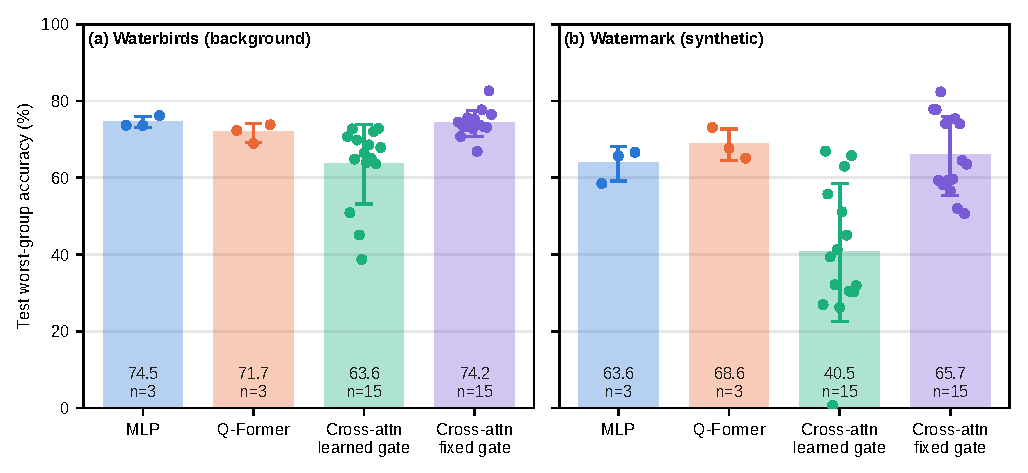
\includegraphics[width=\linewidth]{figures/main_connectors.pdf}
\caption{Test worst-group accuracy of the four connectors (Qwen3.5-4B, SigLIP-base) on (a) Waterbirds and (b) Watermark. Bars are means with one standard deviation; dots are single seeds; hatching distinguishes connectors; the numbers under each bar give the mean and the number of seeds. Only the learnable, zero-start gate fails, and it is also the least stable}\label{fig:main}
\end{figure*}

Fixing the gate raises worst-group accuracy in all four LLM and task cells (Table \ref{tab:h1}, Figure \ref{fig:forest}). The
effects are large (\(d_z\) = 1.10 and 1.34 on Qwen3.5-4B) and every cell survives Holm correction (largest adjusted
\(p\) = 0.009). The result holds when the checkpoint is chosen without group labels (+17.7 and +25.5 points), with
unpaired Welch and Mann--Whitney tests (all \(p \le 0.002\)), and on the confirmation seeds alone (Waterbirds +10.5,
\(p = 9.5 \times 10^{-4}\); Watermark +26.7, \(p = 2.5 \times 10^{-4}\)). The fixed gate also raises average accuracy
(84.1 to 88.0 on Waterbirds, 76.9 to 86.1 on Watermark), so the gain is not a trade against average accuracy.

\begin{table*}[t]
\centering
\caption{Hypothesis H1, paired by seed. One-sided paired t-test at \(\alpha = 0.025\); all four cells survive Holm
correction. Collapsed runs have worst-group accuracy below 50\%. On Phi-4-mini Watermark, seeds 5 to 9 were added
after the 5-seed test missed \(\alpha\) (\(p = 0.044\)); tested alone they give \(p = 0.023\). \label{tab:h1}}
\footnotesize
\begin{tabular}{@{}
  >{\raggedright\arraybackslash}p{(\linewidth - 14\tabcolsep) * \real{0.1053}}
  >{\raggedright\arraybackslash}p{(\linewidth - 14\tabcolsep) * \real{0.1053}}
  >{\centering\arraybackslash}p{(\linewidth - 14\tabcolsep) * \real{0.1316}}
  >{\centering\arraybackslash}p{(\linewidth - 14\tabcolsep) * \real{0.1316}}
  >{\centering\arraybackslash}p{(\linewidth - 14\tabcolsep) * \real{0.1316}}
  >{\centering\arraybackslash}p{(\linewidth - 14\tabcolsep) * \real{0.1316}}
  >{\centering\arraybackslash}p{(\linewidth - 14\tabcolsep) * \real{0.1316}}
  >{\centering\arraybackslash}p{(\linewidth - 14\tabcolsep) * \real{0.1316}}@{}}
\toprule
\begin{minipage}[b]{\linewidth}\raggedright
LLM
\end{minipage} & \begin{minipage}[b]{\linewidth}\raggedright
Task
\end{minipage} & \begin{minipage}[b]{\linewidth}\centering
Seeds
\end{minipage} & \begin{minipage}[b]{\linewidth}\centering
Learnable
\end{minipage} & \begin{minipage}[b]{\linewidth}\centering
Fixed
\end{minipage} & \begin{minipage}[b]{\linewidth}\centering
Gain {[}95\% CI{]}
\end{minipage} & \begin{minipage}[b]{\linewidth}\centering
H1 \(p\)
\end{minipage} & \begin{minipage}[b]{\linewidth}\centering
Collapsed (learnable / fixed)
\end{minipage} \\
\midrule
Qwen3.5-4B & Waterbirds & 15 & 63.6 & 74.2 & +10.6 {[}5.3, 16.0{]} & \(4 \times 10^{-4}\) & 2 / 0 \\
Qwen3.5-4B & Watermark & 15 & 40.5 & 65.7 & +25.2 {[}14.8, 35.6{]} & \(7 \times 10^{-5}\) & 10 / 0 \\
Phi-4-mini & Waterbirds & 5 & 60.4 & 70.1 & +9.7 {[}3.8, 15.7{]} & 0.005 & 0 / 0 \\
Phi-4-mini & Watermark & 10 & 29.4 & 54.9 & +25.5 {[}8.2, 42.7{]} & 0.004 & 8 / 6 \\
\bottomrule
\end{tabular}
\end{table*}

\begin{figure}[t]
\centering
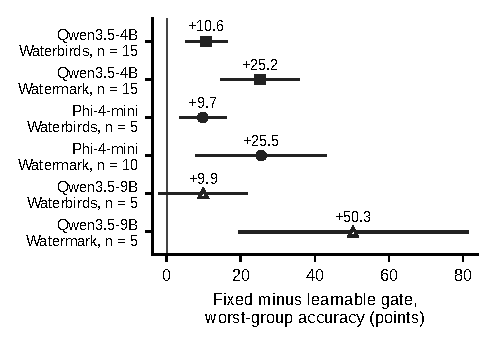
\includegraphics[width=\linewidth]{figures/forest_gain.pdf}
\caption{Paired gain from fixing the gate (fixed minus learnable gate, worst-group accuracy points) with 95\% confidence intervals; squares Qwen3.5-4B, circles Phi-4-mini}\label{fig:forest}
\end{figure}

The learnable gate also makes robustness depend on the seed (H2). On Qwen3.5-4B its variance is higher on both tasks
(variance-ratio \(p = 9 \times 10^{-5}\) and 0.02) and it collapses in 2 of 15 and 10 of 15 runs, against none for
the fixed gate (Figure \ref{fig:seeds}). On Phi-4-mini the variance difference is not significant (\(p\) = 0.20 and
0.23), and on Watermark the fixed gate still collapses in 6 of 10 runs.

\begin{figure*}[t]
\centering
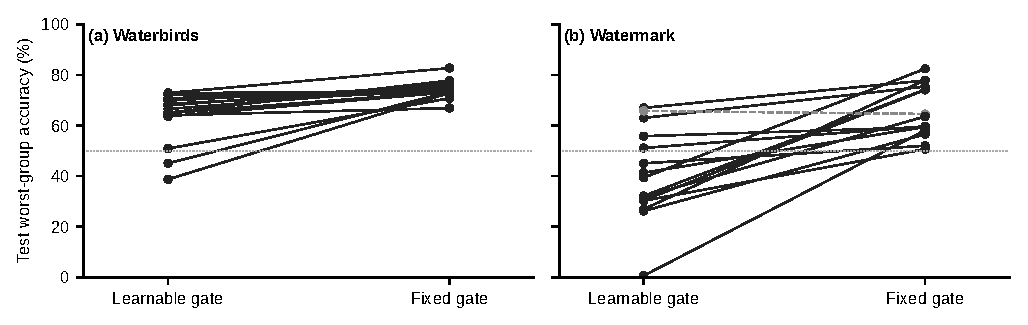
\includegraphics[width=\linewidth]{figures/h1_seeds_qwen.pdf}
\caption{Each line joins one paired run of the learnable gate to the fixed gate (Qwen3.5-4B) on (a) Waterbirds and (b) Watermark. Solid lines rise and dashed lines fall; the dotted line marks the 50\% collapse threshold}\label{fig:seeds}
\end{figure*}

\subsection{The zero start, not learnability, is the cause}

Controls change one property of the learnable gate at a time (Table \ref{tab:controls}; all exploratory).

\begin{table*}[t]
\centering
\caption{Controls on Qwen3.5-4B, test worst-group accuracy (\%), Waterbirds / Watermark unless stated. \label{tab:controls}}
\footnotesize
\begin{tabular}{@{}
  >{\raggedright\arraybackslash}p{(\linewidth - 8\tabcolsep) * \real{0.1739}}
  >{\centering\arraybackslash}p{(\linewidth - 8\tabcolsep) * \real{0.2174}}
  >{\centering\arraybackslash}p{(\linewidth - 8\tabcolsep) * \real{0.2174}}
  >{\centering\arraybackslash}p{(\linewidth - 8\tabcolsep) * \real{0.2174}}
  >{\raggedright\arraybackslash}p{(\linewidth - 8\tabcolsep) * \real{0.1739}}@{}}
\toprule
\begin{minipage}[b]{\linewidth}\raggedright
Control
\end{minipage} & \begin{minipage}[b]{\linewidth}\centering
Seeds
\end{minipage} & \begin{minipage}[b]{\linewidth}\centering
Learnable variant
\end{minipage} & \begin{minipage}[b]{\linewidth}\centering
Reference
\end{minipage} & \begin{minipage}[b]{\linewidth}\raggedright
What it shows
\end{minipage} \\
\midrule
Learnable gate started open (\(\tanh\alpha_0 = 0.995\)) & 5 & 71.8 / 66.8 & fixed 72.9 / 72.1 & starting open removes most of the gap \\
Fixed gate with injection capped at the text norm & 5 & 69.9 / 50.6 & zero start 61.2 / 42.6; fixed 73.1 / 67.2 & keeps part of the gain on Waterbirds (\(-3.2\) against fixed, \(p\) = 0.13) but loses most on Watermark (\(-16.6\), \(p\) = 0.002); 2 of 5 Watermark seeds collapse \\
Learnable gate started at \(\tanh\alpha_0 = 0.01\) & 5 & 69.1 / 22.5 & zero start 61.2 / 42.6; fixed 73.1 / 67.2 & gate falls back to 0.001 to 0.008; Watermark collapses in 5 of 5 seeds, \(-20.1\) below the zero start (\(p\) = 0.041) \\
Learnable gate started at \(\tanh\alpha_0 = 0.1\) & 5 & 73.1 / 65.3 & zero start 61.2 / 42.6; fixed 73.1 / 67.2 & +11.9 and +22.7 over the zero start (\(p\) = 0.041, 0.072); no difference from the fixed gate \\
Learnable gate started half open (\(\tanh\alpha_0 = 0.5\)) & 5 & 72.6 / 62.7 & zero start 61.2 / 42.6; fixed 73.1 / 67.2 & +11.4 and +20.1 over the zero start (\(p\) = 0.014, 0.006); no difference from the fixed gate \\
Gate excluded from gradient clipping & 3 & 67.2 / 52.9 & zero start, same seeds 64.4 / 39.3 & no significant change; gate stays below 0.003 \\
No weight decay on the gate & 2 & 52.2 / 28.0 & zero start, same seeds 60.9 / 44.9 & no rescue \\
Connector learning rate \(5 \times 10^{-5}\) / \(2 \times 10^{-4}\) / \(10^{-3}\) (Waterbirds) & 2 & 35.9 / 56.8 / 65.8 & fixed 65.6 / 73.5 / 66.5 & the gap shrinks as the gate moves further (final 0.002 / 0.004 / 0.018) \\
fp16 weights instead of 4-bit & 3 & 63.2 / 44.1 & fixed 73.2 / 65.1 & same direction (+10.0, +21.1; not significant with 3 seeds) \\
Eight training epochs (Waterbirds) & 4 & 67.9 & fixed 79.0 & +11.0 (\(p\) = 0.023); one of five fixed-gate runs collapsed \\
\bottomrule
\end{tabular}
\end{table*}

A learnable gate that starts half open behaves like the fixed gate and moves little (final \(\tanh\alpha\) 0.44),
so the outcome depends on where the gate starts rather than on whether it can learn. A start of 0.1 is already
enough. That gate shrinks during training, to 0.058 to 0.064, but stays about a hundred times above the zero-start
gate, and its worst-group accuracy equals the fixed gate's on Waterbirds (73.1 against 73.1). Its gradient also
changes sign often: 27\% to 51\% of steps per epoch push the gate up, with a slight net push down. A start of 0.01
is not enough. That gate falls back to the zero-start range (final \(|\tanh\alpha|\) 0.001 to 0.008), and Watermark
collapses below 50\% in all five seeds (22.5, against 42.6 for the zero start). Because this control also starts
\(W_o\) at zero, the gradient of \(W_o\) is scaled by the small gate, which may explain why it ends below the zero
start. The threshold therefore lies between 0.01 and 0.1. Ten times longer alignment
leaves the zero-start gate below 0.003 but also destabilises the learnable-gate alignment (caption loss rises from
2.0 to 7.9), so that run shows fragility rather than a clean effect and is reported only in the supplement.

\subsection{The gate's gradient is large but cancels itself}

After alignment the zero-start gate sits at \(|\tanh\alpha| \approx 0.0005\) and never exceeds 0.01. Its gradient is
not small: the mean absolute pre-clipping gradient per epoch ranges from 3 to 1,528 across 13 learnable-gate runs,
and in some runs it is almost all of the global gradient norm. With Adam, each step moves \(\alpha\) by at most about
the learning rate \(\eta = 2 \times 10^{-4}\), so over the roughly 900 to 1,200 task steps a gradient of constant sign
would move \(\alpha\) by up to about 0.2. The observed change is below 0.003. The gradient must therefore change sign
from step to step and cancel. The signed gradient, logged in seven further zero-start runs, confirms this: the mean
absolute gradient reaches 37 to 1,282 per epoch, yet 37\% to 60\% of steps push the gate up, the sign changes on 45\%
to 49\% of consecutive steps, and the gate ends at 0.001 to 0.005. The gate started at 0.01 behaves the same way
(30\% to 58\% of steps push it up). This differs from the dead-gradient account of \citep{farazi2026gate}, which requires an
injected signal that does not depend on the text; ours does.

\subsection{The pathway is weak, not closed}

The learnable gate passes 15 to 35 times less visual signal than the fixed gate (injection ratio 3.5 against 112,
6 runs each), because \(W_o\) grows to partly offset the small gate. Removing the visual pathway at inference, or
zeroing the image features, makes the learnable-gate model give the same answer to every image in every run:
average accuracy falls from 83.0 to the share of one class on Waterbirds (\(-46.9\) points, 4 of 4 seeds, \(p\) = 0.035)
and from 81.8 to 50.0 on Watermark (3 of 3 seeds, \(p\) = 0.003). The fixed-gate model does the same. The learnable
gate therefore still uses the image; its pathway is weak, not closed. In these runs the fixed gate again led on
worst-group accuracy (+16.2 on Waterbirds, 4 seeds; +14.4 on Watermark, 3 seeds). Within learnable-gate runs the injection ratio does not predict
worst-group accuracy (Spearman \(\rho\) = 0.33, \(p\) = 0.27). Both gate variants attend to the watermark corner more
than to the rest of the image (16.7\% and 18.2\% of attention against 8.2\% if uniform), yet only the learnable-gate
model relies on it.

\subsection{Connector type matters little once the gate is fixed}

MLP projector and Q-Former do not differ significantly (5 seeds; \(p\) = 0.23 on Waterbirds and 0.40 on Watermark),
and neither differs significantly from the fixed gate, although equivalence within three points is not established.
Matching the number of image tokens (36 instead of 49 MLP tokens) changes nothing (74.7 against 74.9). The fixed-gate
connector needs about half the step time and memory of the MLP projector (1.7 against 4.0 s per step; 6.2 against
12.1 GB on one T4).

\subsection{Boundaries of the effect}

\emph{Injection depth.} With four gated blocks inside the decoder, the learnable and fixed gates do not differ (Waterbirds
70.8 against 70.4, 5 seeds; Watermark 68.3 against 70.6, 4 seeds), although the per-layer learnable gates also stay
small (mean \(|\tanh\alpha|\) 0.027).

\emph{Encoder size.} With SigLIP-large every connector improves on Waterbirds by 6 to 11 points, and the gap narrows to
+8.0 (\(p\) = 0.09, 4 paired seeds). On Watermark it remains: 53.2 against 75.6 (+22.4, \(d_z\) = 0.85, \(p\) = 0.13,
5 seeds) (Figure \ref{fig:encoder}).

\emph{Third task.} On CelebA the direction is the same but not significant (43.5 against 51.1, +7.7, \(p\) = 0.48, 5 paired
seeds).

\emph{Shortcut strength.} At a 90\% watermark correlation all arms learn the task (learnable 75.7, fixed 77.5); at 99\% all
arms fail (6.7 and 20.1). The gap is largest at the 95\% used in the main experiment.

\emph{Group labels.} Group distributionally robust optimisation (Group DRO) \citep{sagawa2020groupdro}, which uses group labels in training, closes the gap on Waterbirds (+2.3, \(p\) = 0.70,
4 seeds) but not on Watermark (+17.5, \(p\) = 0.059).

\begin{figure*}[t]
\centering
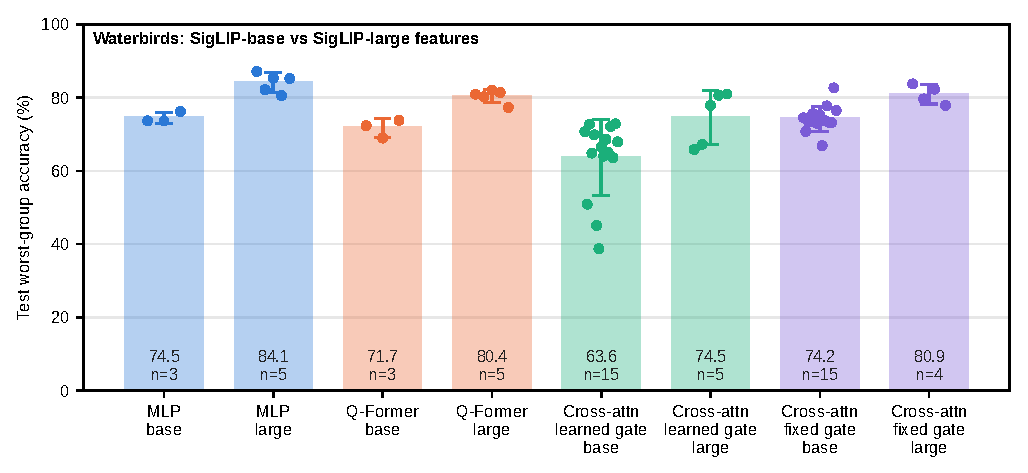
\includegraphics[width=\linewidth]{figures/encoder_scale.pdf}
\caption{Waterbirds worst-group accuracy with SigLIP-base and SigLIP-large features. Bars are means with one standard deviation, dots are single seeds, and the numbers under each bar give the mean and the number of seeds. Every connector gains from the larger encoder; the learnable gate still lags}\label{fig:encoder}
\end{figure*}

\subsection{Free-form answers under shifted priors}

On VQA-CP v2 every model loses 15 to 21 points when the answer priors shift, so the subset exposes the language
prior (Table \ref{tab:vqacp}). A text-only model with the same LLM, LoRA and budget sets the reference. The learnable gate does no
better than this model in distribution (47.6 against 48.2, \(p\) = 0.23), and removing its visual pathway changes
nothing, so it does not use the image at test time (injection ratio 0.05). Its 2.1-point lead under shifted priors
(\(p\) = 0.041) remains with the image removed (29.2), so it comes from training with the pathway present rather
than from the test image. The fixed gate is worse than having no image at all: \(-5.7\) points in distribution
against the text-only model (\(p\) = 0.001). Its injected signal is about 70 times the text norm, and removing it
raises shifted-prior accuracy by 4.6 points.

Capping the injected signal at the text norm removes this cost. The capped connector scores 49.6 in distribution and
30.6 under shifted priors, 7.0 points above the uncapped fixed gate in distribution (\(p\) = 0.020) and 3.5 points
above the text-only model under shifted priors (\(p\) = 0.028). It is also the only model whose accuracy depends on
the test image: removing the pathway or zeroing the image features costs 2.8
to 3.5 points in distribution and 1.0 to 2.0 under shifted priors (\(p\) = 0.041 to 0.063, 3 seeds). Strong injection
therefore disturbs free-form generation, and an injection held at the text norm avoids that while still using the
image. On the binary shortcut tasks, however, the cap gives back much of the fixed gate's gain (Table \ref{tab:controls}): Waterbirds
69.9 against 73.1 for the uncapped fixed gate (\(p\) = 0.13) and Watermark 50.6 against 67.2 (\(p\) = 0.002, \(d_z\) =
\(-3.1\)), with two of five Watermark seeds collapsed. The capped model still uses the image on these tasks: removing
the pathway makes it give one answer to every image. Injection strength therefore trades shortcut robustness on a
class readout against the quality of free-form answers.

\begin{table*}[t]
\centering
\caption{VQA-CP v2 subset, VQA accuracy (\%), mean ± standard deviation over 3 seeds. Prior answer rate: share of answers
equal to the most frequent training answer for the question type (same priors / shifted priors). Not comparable with
published VQA-CP results. \label{tab:vqacp}}
\footnotesize
\begin{tabular}{@{}
  >{\raggedright\arraybackslash}p{(\linewidth - 12\tabcolsep) * \real{0.1176}}
  >{\centering\arraybackslash}p{(\linewidth - 12\tabcolsep) * \real{0.1471}}
  >{\centering\arraybackslash}p{(\linewidth - 12\tabcolsep) * \real{0.1471}}
  >{\centering\arraybackslash}p{(\linewidth - 12\tabcolsep) * \real{0.1471}}
  >{\centering\arraybackslash}p{(\linewidth - 12\tabcolsep) * \real{0.1471}}
  >{\centering\arraybackslash}p{(\linewidth - 12\tabcolsep) * \real{0.1471}}
  >{\centering\arraybackslash}p{(\linewidth - 12\tabcolsep) * \real{0.1471}}@{}}
\toprule
\begin{minipage}[b]{\linewidth}\raggedright
Model
\end{minipage} & \begin{minipage}[b]{\linewidth}\centering
Test, same priors
\end{minipage} & \begin{minipage}[b]{\linewidth}\centering
Image removed
\end{minipage} & \begin{minipage}[b]{\linewidth}\centering
Test, shifted priors
\end{minipage} & \begin{minipage}[b]{\linewidth}\centering
Image removed
\end{minipage} & \begin{minipage}[b]{\linewidth}\centering
Prior answer rate
\end{minipage} & \begin{minipage}[b]{\linewidth}\centering
Injection ratio
\end{minipage} \\
\midrule
Text only & 48.2 ± 0.4 & n/a & 27.1 ± 0.1 & n/a & 39.9\% / 35.0\% & 0 \\
Learnable gate & 47.6 ± 0.2 & 47.6 ± 0.2 & 29.1 ± 0.8 & 29.2 ± 0.7 & 39.9\% / 33.2\% & 0.05 \\
Fixed gate & 42.6 ± 0.7 & 40.4 ± 0.9 & 27.6 ± 0.8 & 32.2 ± 0.4 & 33.8\% / 31.1\% & 70.1 \\
Capped injection & 49.6 ± 1.7 & 46.7 ± 0.4 & 30.6 ± 0.9 & 29.7 ± 1.2 & 39.0\% / 32.7\% & 1.00 \\
\bottomrule
\end{tabular}
\end{table*}

\subsection{A connector-only fix}

Retraining only the connector on half of the group-balanced validation set, with the LLM and LoRA frozen, lifts the
fixed-gate connector on Watermark from 72.5 to 89.6 ± 0.5 (5 seeds). This beats the same fix on the MLP projector
(81.2; +8.4, \(p < 0.001\)) and a linear probe trained the same way on the frozen features (85.1). On Waterbirds it
gives no gain (73.9 to 74.1) (Figure \ref{fig:fixes}). Qwen3.5-4B with its own vision tower, zero-shot and with a
threshold calibrated on validation, reaches only 35.5 on Waterbirds.

\begin{figure*}[t]
\centering
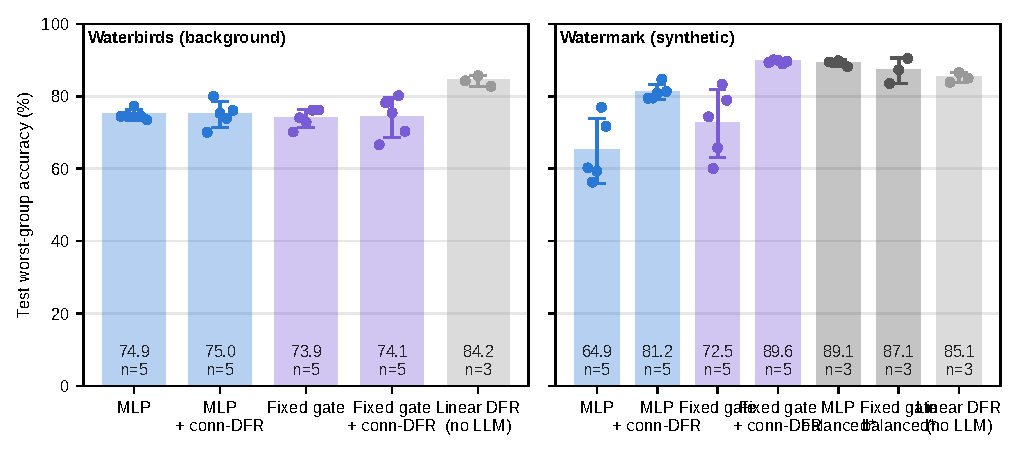
\includegraphics[width=\linewidth]{figures/fixes.pdf}
\caption{Connector-only deep feature reweighting (conn-DFR), group-balanced sampling and a linear probe on the frozen features. Bars are means with one standard deviation, dots are single seeds, and the numbers under each bar give the mean and the number of seeds; (a) Waterbirds, (b) Watermark. Starred bars use group labels during training (group-balanced sampling). Conn-DFR on the fixed gate reaches 89.6\% worst-group accuracy on Watermark and gives no gain on Waterbirds}\label{fig:fixes}
\end{figure*}

\subsection{Gates in released models}

The released weights of models that use the same zero-start tanh gates show the same regime. Nine of the 20
cross-attention gates of IDEFICS-80B have \(|\tanh\alpha| < 0.05\), and so do all gates of Llama 3.2 11B Vision (8 of 8)
and 90B Vision Instruct (20 of 20), whose values are at most 0.012. A small gate does not show that these models
ignore the image; we did not test them for shortcut reliance.


\section{Discussion}\label{sec:discussion}
\subsection{A transmission account of shortcut reliance}

Work on spurious correlations in classifiers concludes that features usually carry the core signal and that the
readout decides whether it is used \citep{izmailov2022feature,kirichenko2023dfr}. Our results add a stage between the two:
the connector decides how much of the feature signal reaches the readout. With a zero-start learnable gate, the
injected visual signal is an order of magnitude weaker, and the LLM falls back on the cue that is easiest to read
from what remains. A linear probe on the same frozen features reaches 84 to 85 worst-group accuracy with reweighting,
above every vision-language model trained with plain empirical risk minimisation on those features, which confirms that the information is present in the features and is lost on the way to
the readout. This is a concrete case of modality under-use \citep{wu2022greedy,huang2022modality} located in one component
that ships in released models.

\subsection{Relation to gate closure in frozen VLMs}

Farazi et al.~find that learnable gates on image-derived pathways in frozen VLMs settle near zero and that the
pathways become behaviourally closed, and they explain it by a first-order gradient that vanishes when the injected
signal does not depend on the caption \citep{farazi2026gate}. Our connector is text-coupled, the case they leave open. Its
gate also stays near zero, but through a large gradient that cancels itself, and its pathway is still used. Both
results agree that a gate's value is not evidence of how much the pathway is used, in either direction. They differ on
what the small gate does: in our setting it does not remove the image, it weakens it enough for a shortcut to win.

\subsection{Initialisation and injection strength must be chosen together}

A non-zero start, as LayerScale recommends for optimisation \citep{touvron2021cait} and as recent connectors already use
\citep{lialin2023scalable,yan2026dgp}, removes the robustness cost of the gate. Standard fixes do not reliably remove it:
connector-level DFR rescued the zero-start gate on the watermark task but not on Waterbirds, and JTT on neither, so
the start value should be set at design time rather than repaired afterwards.
Strong injection has its own cost: the fixed gate injects about 70 to 130 times the text-embedding norm, which helps
the binary readout but disturbs free-form answers on VQA-CP, where it scores below a text-only model. This matches
reports that visual tokens with much larger norms than text tokens lose information in pre-norm MLLMs
\citep{li2025unseen} and the advice to inject at a matched norm \citep{farazi2026gate}. Capping the injection at the text norm
repairs generation in our connector: the capped model is the best on both VQA-CP test splits and the only one whose
answers depend on the test image. The same cap, however, gives back most of the robustness gain on the watermark
task at 4B (50.6 against 67.2), although with the 9B model it kept the gain (63.9 against 63.2), so the cost may
shrink with scale. Neither earlier study measures shortcut reliance, so this cost of norm matching was not
visible to them. In our data a strong visual signal is what lets the class readout override a textual or
background shortcut, and the same strength disturbs free-form decoding. No single injection strength was best on
both kinds of task, so the strength should be chosen for the output the model must produce, and robustness should
be measured whenever it is changed.

\subsection{Why per-layer gates behave differently}

With four gated blocks at different depths, the learnable and fixed gates do not differ. The per-layer learnable gates
end about seven times larger than the single input-level gate (mean 0.027 against 0.0037), and four routes into the
decoder give the image several chances to contribute. The effect we report therefore belongs to the single
input-level design, as used in adapter-style injection, and not to every gated architecture.

\subsection{Attention is not reliance}

Both gate variants attend to the watermark corner about twice as much as a uniform map would, yet only the
learnable-gate model fails on images where the watermark and the label disagree. Attention maps alone would not have
separated the two models \citep{jain2019attention,wiegreffe2019attention}; the pathway test and the group-level accuracies
did.


\section{Practical and societal implications}\label{sec:implications}
\subsection{For model builders}

When a modality is injected into a pretrained LLM through a learnable gate, the gate should not start at or near zero:
in our experiments a start of 0.01 was too small and 0.1 was enough. A fixed gate with a zero-initialised output
layer, or a learnable gate that starts at 0.1 or higher with a zero-initialised output layer, keeps the identity at
initialisation and removed the robustness cost. This costs nothing: no group labels, no extra
training and no extra compute. A learnable gate that is kept should be logged during training, and the injected
signal should be checked against the text-embedding norm: a very strong injection harmed free-form generation, but
capping it at the text norm cost most of the robustness gain on the watermark task, so the norm must be tuned for
the intended output and robustness re-measured when it changes. When a small group-balanced set exists, retraining only the connector is a cheap fix for localised
shortcuts such as watermarks.

\subsection{For evaluation}

A connector comparison on one or three seeds can point the wrong way: on Watermark the learnable gate's worst-group
accuracy ranged from 0.7\% to 66.9\% across 15 seeds. Architectural robustness claims should report worst-group accuracy over at
least five to ten seeds, the number of collapsed runs, and the gate values of any learnable gates.

\subsection{For society}

In medical imaging, shortcut reliance in deep models has already caused failures that stayed hidden until the models
were tested outside their training conditions \citep{degrave2021covid,brown2023shortcut}. Vision-language models inherit
the same risk. Those failures fall on the groups that are rare in training, which makes them a fairness problem
as well as an accuracy problem \citep{ongly2024shortcut}. Our results show that one routine architectural default can make
such failures more likely, and that a cost-free change to the same component reduces the risk without collecting
group labels. The experiments ran on single commodity GPUs with 4B- and 9B-parameter models, so the checks we recommend are
within reach of groups without large compute budgets. The work uses only public datasets and releases code and
results, and we see no new misuse risk from a finding about initialisation.


\section{Limitations}\label{sec:limitations}
All training ran on free Kaggle sessions with two 16 GB T4 GPUs, which set the scale of the study. The confirmatory
tests use 4B-parameter models; the 9B replication is exploratory, with five paired seeds per task, and its Waterbirds
interval includes zero. All models run in 4-bit with LoRA, with a frozen vision encoder and a short alignment of 300
steps. A lower alignment learning rate shrank the Waterbirds gap to between 3 and 9 points and the Watermark gap
at 300 steps to 9.8, and longer alignment did not shrink it further, so the size of the effect depends on the
alignment settings. The LoRA-rank and training-set-size controls have three seeds each. Released gated models are
larger, trained for longer and update their encoders, so our results show a risk in this low-budget regime, not a
property of every gated model. The effect is limited to a single input-level gated block: per-layer gates showed no
gap.

Three of the four tasks use a binary readout from the first answer token. On the one open-ended benchmark, a VQA-CP v2
subset with three seeds, the gate effect did not appear, strong injection hurt generation, and only the capped
connector used the test image beyond a text-only baseline; with three seeds these results are exploratory.

Several controls have few seeds: the pathway ablation three to four, the DFR and JTT comparison on both gates three,
the learning-rate sweep two per setting, fp16 and the shortcut-strength sweep two or three. They are reported as exploratory. Phi-4-mini Watermark was extended from five to
ten seeds after its first test, which we disclose; the added seeds also pass on their own. Runs are not
bit-reproducible on GPUs, so seeds are random replicates rather than exact repeats.

The learnable and fixed gates differ in two ways, whether the gate trains and whether the zero start sits in the gate
or in the output layer. The second difference cannot be removed, because both at zero cannot train; the 0.01 and
0.1 starts with the default \(W_o\) separate them (five seeds each). The open gate barely moves because its
gradient is scaled by \(1 - \tanh^2\alpha \approx 0.01\).

Equivalence between connector types is not established. CelebA uses an 8,000-image training subsample and a binary,
annotator-assigned ``Male'' attribute, so its results say nothing about sex or gender beyond that label; the watermark
shortcut is partly textual \citep{materzynska2022disentangling}, and SigLIP's web pre-training may include images from the
source datasets, a factor shared by every arm. Group DRO is the only full-model group-robust baseline we ran; DFR
and JTT retrain only the connector. We did not run gradient-modulation methods for modality imbalance
\citep{peng2022balanced}, which balance two separately encoded modalities fused at the output and have no direct
counterpart in a model where the image enters the LLM's input, because the study isolates a cause rather than
competing with fixes. Two of the tasks are standard but small
group-robustness benchmarks and one is synthetic; open-ended spurious-cue benchmarks for MLLMs
\citep{ye2026mmspubench,yang2025spuriverse} need a different training protocol and are left to future work. A first version
of the control that gives each test example another example's image swapped images only within a group, because the
test files are stored group by group; it was rerun with a random order, and only the rerun is reported.


\section{Conclusion}\label{sec:conclusion}
Holding the LLM, features, data and training budget fixed, we varied only the connector of an LLM-based vision-language
model. A learnable injection gate that starts at zero lowered worst-group accuracy by 10.6 and 25.2 points on
Qwen3.5-4B and by 9.7 and 25.5 points on Phi-4-mini, and made robustness depend on the seed. With Qwen3.5-9B the
gaps were 9.9 and 50.3 points. Connector-level DFR removed the gap on the watermark task but not on Waterbirds. A gate that starts at
0.1 or higher came close to a fixed gate, while one started at 0.01 fell back near zero, so a start at
or near zero is the cause. The gate stays small because its large gradient
cancels itself, not because the gradient vanishes, and the visual pathway stays weak rather than closed. The effect
did not appear with per-layer gates or on open-ended VQA-CP answers, where strong injection hurt generation. Capping the
injection at the text norm gave the best free-form answers but gave back most of the robustness gain on the
watermark task at 4B (not at 9B), so injection strength can trade one kind of reliability against the other. All experiments ran on free T4 GPUs. Future work should test released gated models and larger models trained for longer
and benchmarks of spurious cues for
open-ended answers \citep{ye2026mmspubench,yang2025spuriverse}.


\backmatter

\bmhead{Acknowledgements}
The experiments ran on free GPU notebooks provided by Kaggle.

\section*{Statements and Declarations}

\bmhead{Funding}
The authors did not receive support from any organization for the submitted work.

\bmhead{Competing interests}
The authors have no relevant financial or non-financial interests to disclose.

\bmhead{Ethics approval}
Not applicable. The study involves no new data from human participants and no animals; it uses only public datasets
(Waterbirds, COCO 2017, CelebA, VQA-CP v2) under their licences, and Waterbirds and CelebA are licensed for
non-commercial research.

\bmhead{Consent to participate}
Not applicable.

\bmhead{Consent for publication}
Not applicable. The article reproduces no image of an identifiable person; CelebA face images were used only for
training and testing.

\bmhead{Data availability}
Waterbirds, COCO 2017, CelebA and VQA-CP v2 are publicly available from their original sources. The scripts that
rebuild every split, and the results of every training run (per-run metrics and per-example predictions), are in the
code repository below. The per-run results behind every table and figure are also provided as Online Resource 1.

\bmhead{Code availability}
\url{https://github.com/Naveenvaidani/VLM-Debias} (code, job scripts and pinned package versions). A licence must be
added before submission.

\bmhead{Use of AI tools}
Described in the Methods section (Use of AI tools), as the journal requires.

\bmhead{Dual use}
The work concerns a training default of vision-language models and has no identified dual-use risk.

\bmhead{Author contributions}
Both authors contributed equally to conceptualization, methodology, software, investigation, formal analysis,
visualization, writing of the original draft, and review and editing. Both authors read and approved the final
manuscript.

\bmhead{ORCID}
Jeyadev R: \url{https://orcid.org/0009-0005-5854-390X}; Naveen SomaSekhar Varma Vaidani:
\url{https://orcid.org/0009-0008-7082-9937}.

\bibliography{references}

\end{document}
